\begin{landscape}
% \thispagestyle{empty}
\section{Schematics}


\subsection{Gas System}
\begin{figure}[H]
    \centering
    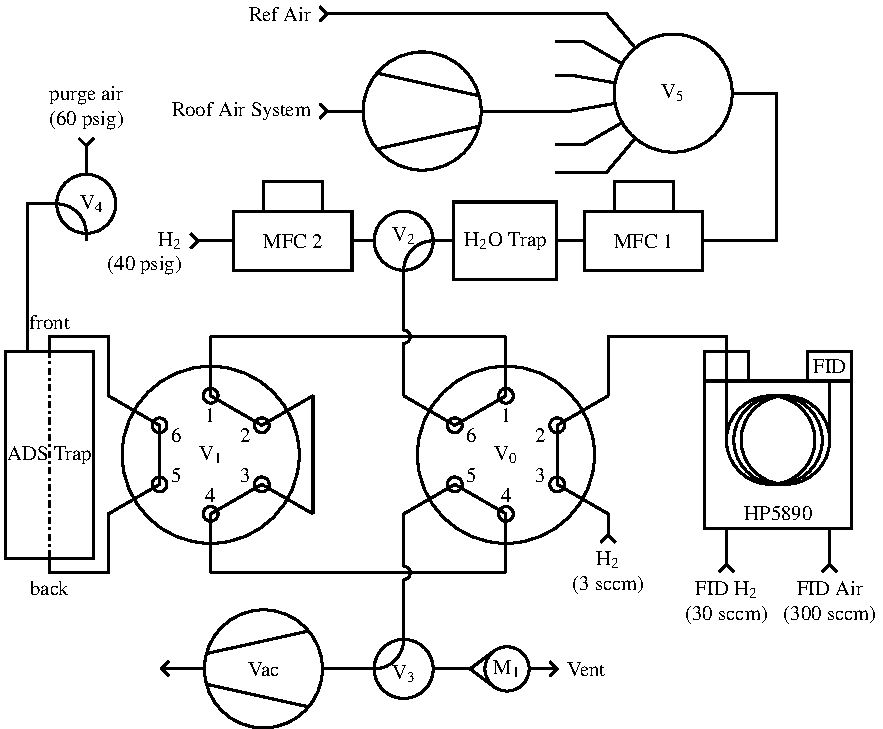
\includegraphics[]{Figures/Pre-Concentration States/Default.pdf}
    \caption{Pre-Concentration system in the sampling configuration.}
    \label{fig:Pre-Con Sampling}
\end{figure}


\subsection{System Power}
\pagebreak


\subsection{GC Remote and Manual Overrides}
\begin{figure}[H]
    \centering
    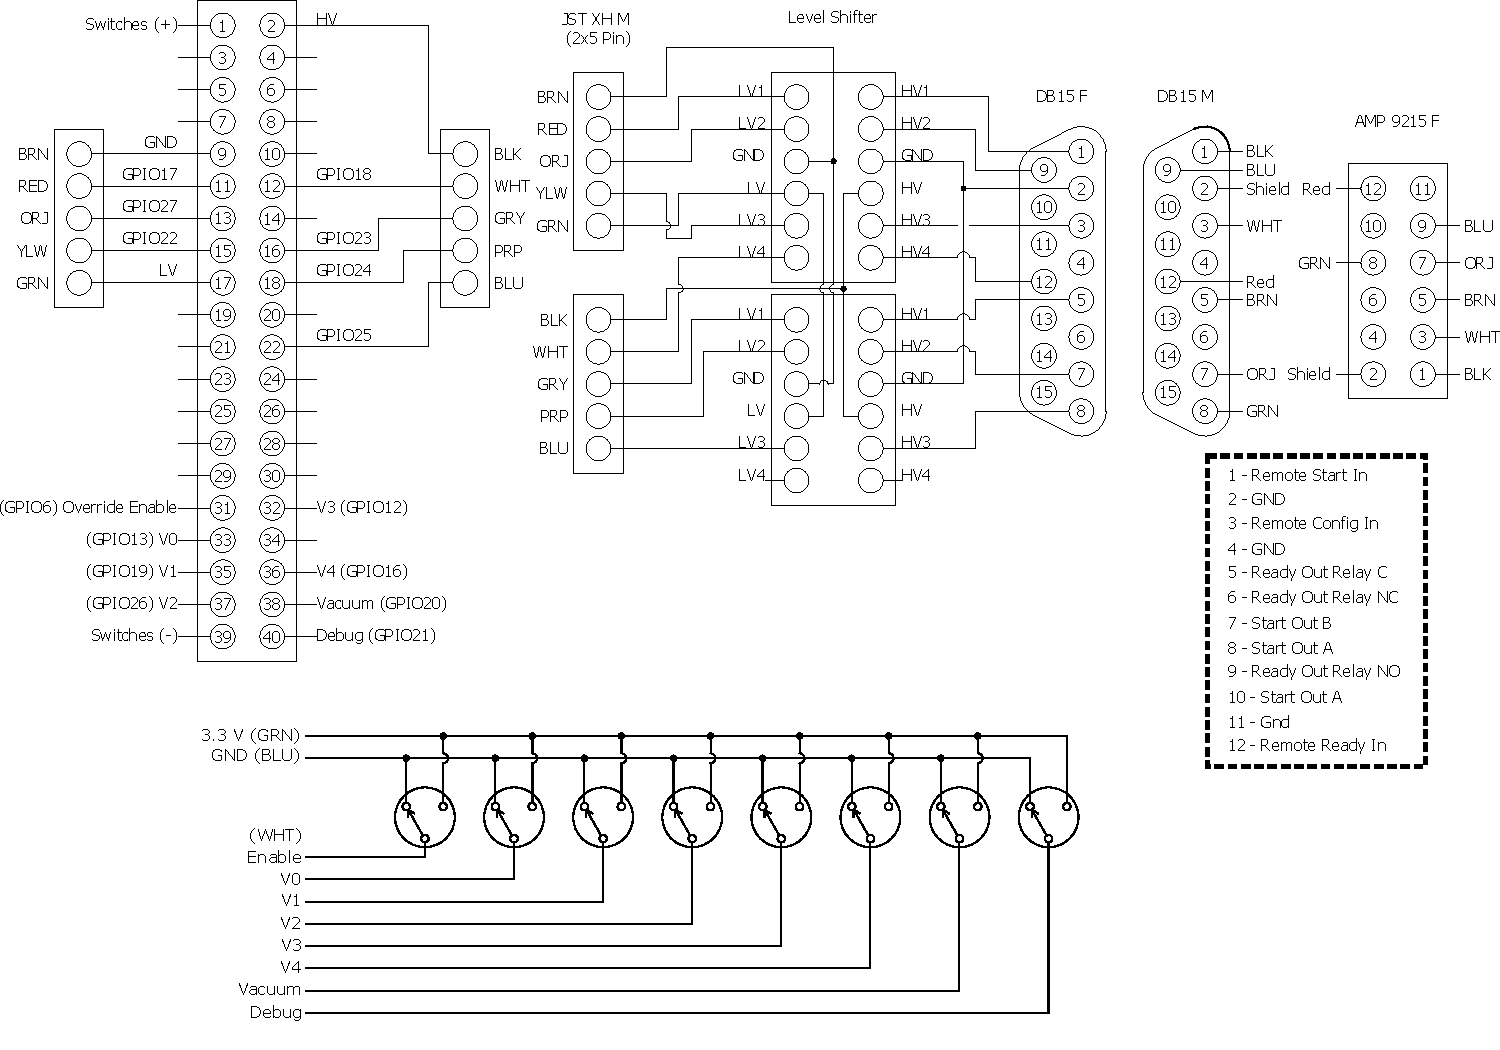
\includegraphics[width=0.9\linewidth]{Figures/RPi GPIO Schematic.pdf}
    \caption{Connections for the GC remote control cable.}
    \label{fig: GC remote}
\end{figure}


\subsection{Mass Flow Controller}
\begin{figure}[H]
    \centering
    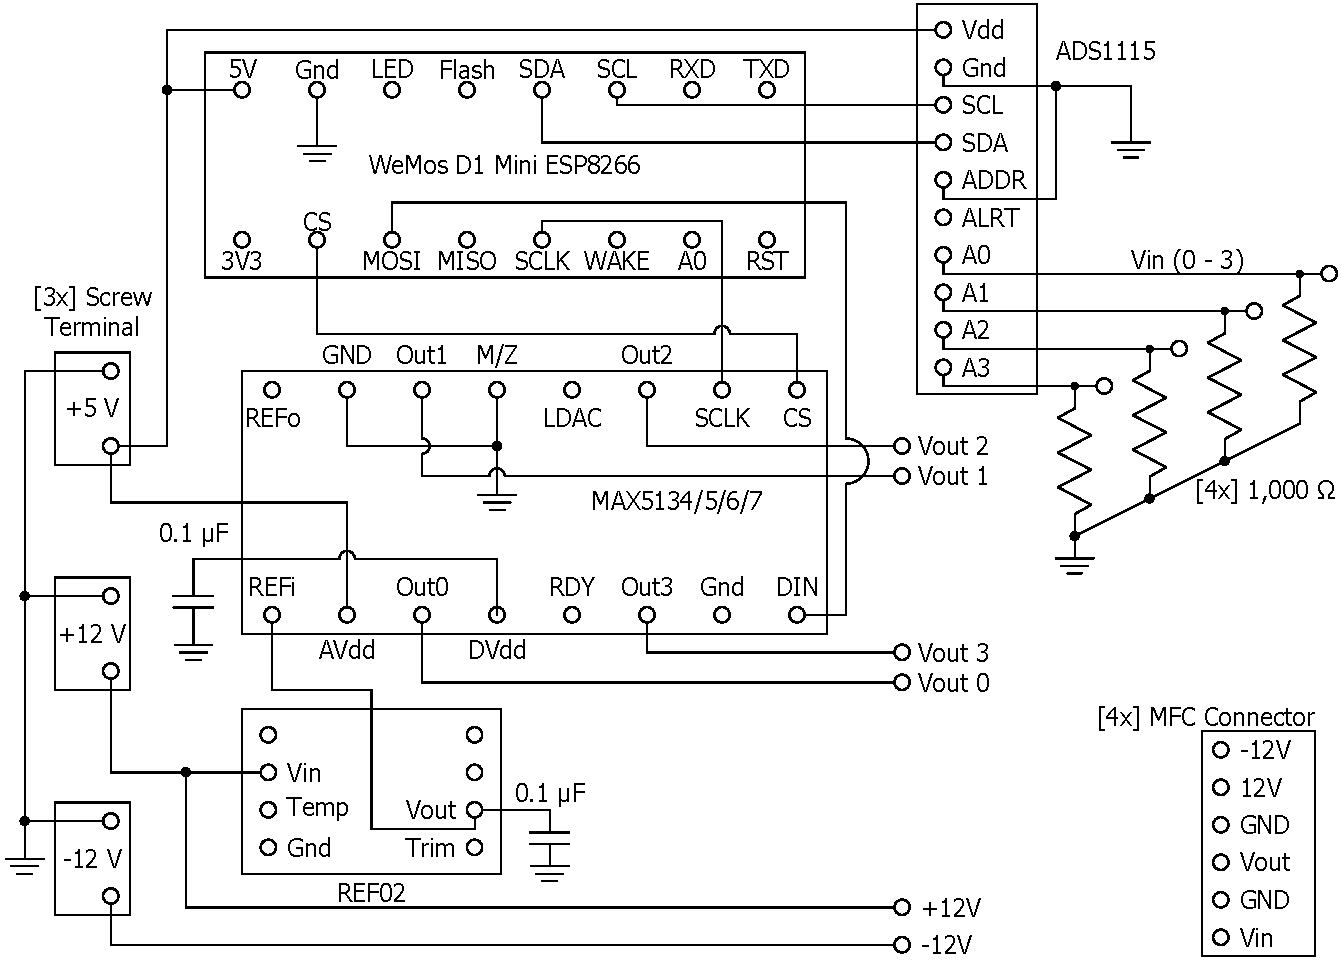
\includegraphics[width=0.875\linewidth]{Figures/MFC Controller.pdf}
    \caption{Mass Flow Controller electrical diagram.}
    \label{fig: MFC electronics}
\end{figure}


\subsection{Valve Controller}
\begin{figure}[H]
    \centering
    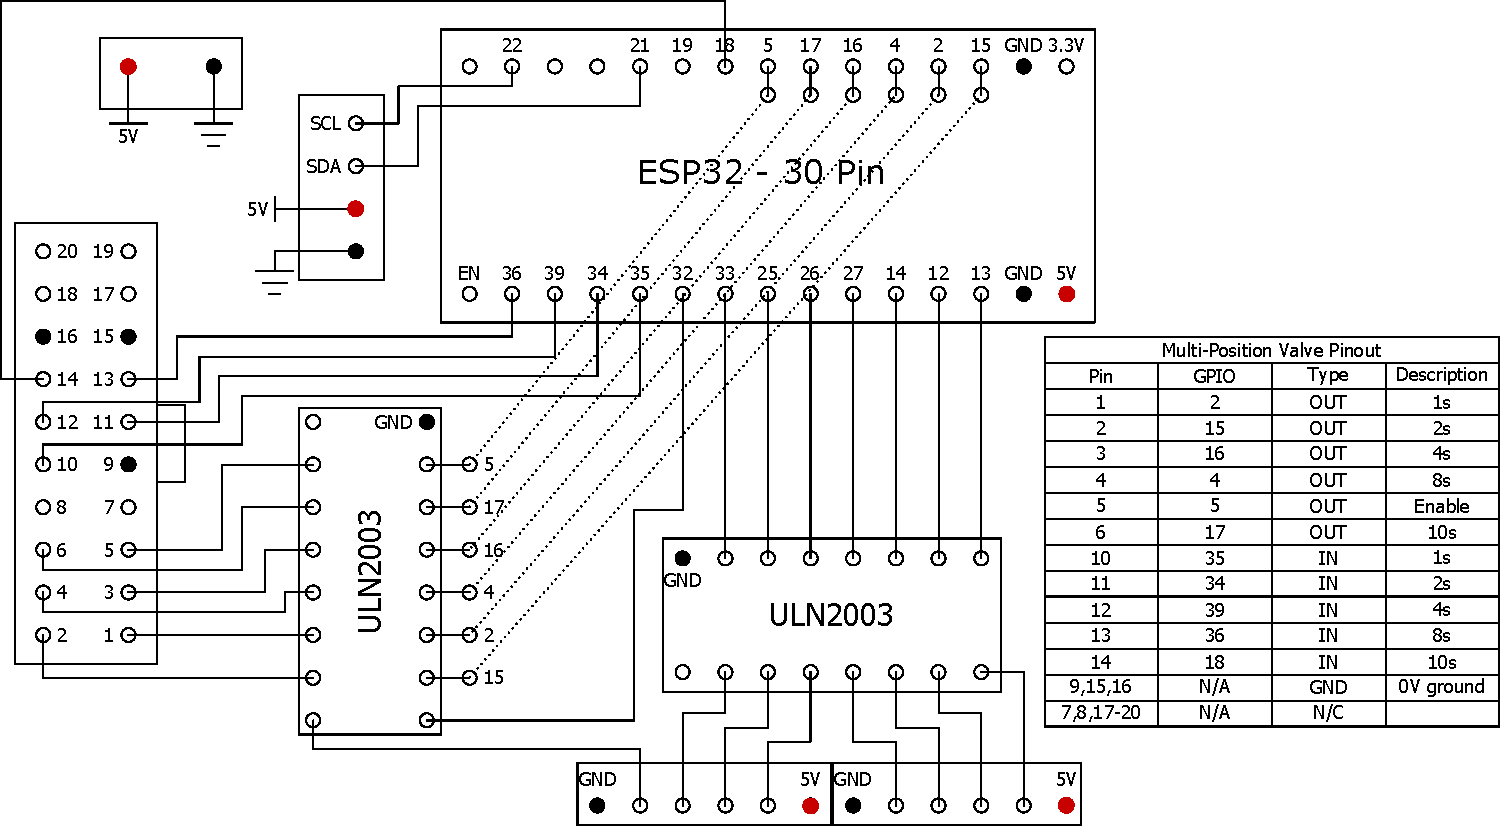
\includegraphics[width=0.9\linewidth]{Figures/Valve Controller Schematic.pdf}
    \caption{Valve controller electrical diagram}
    \label{fig:fig: valve controller}
\end{figure}


\subsection{Adsorbent Trap Heater}
\begin{figure}[H]
    \centering
    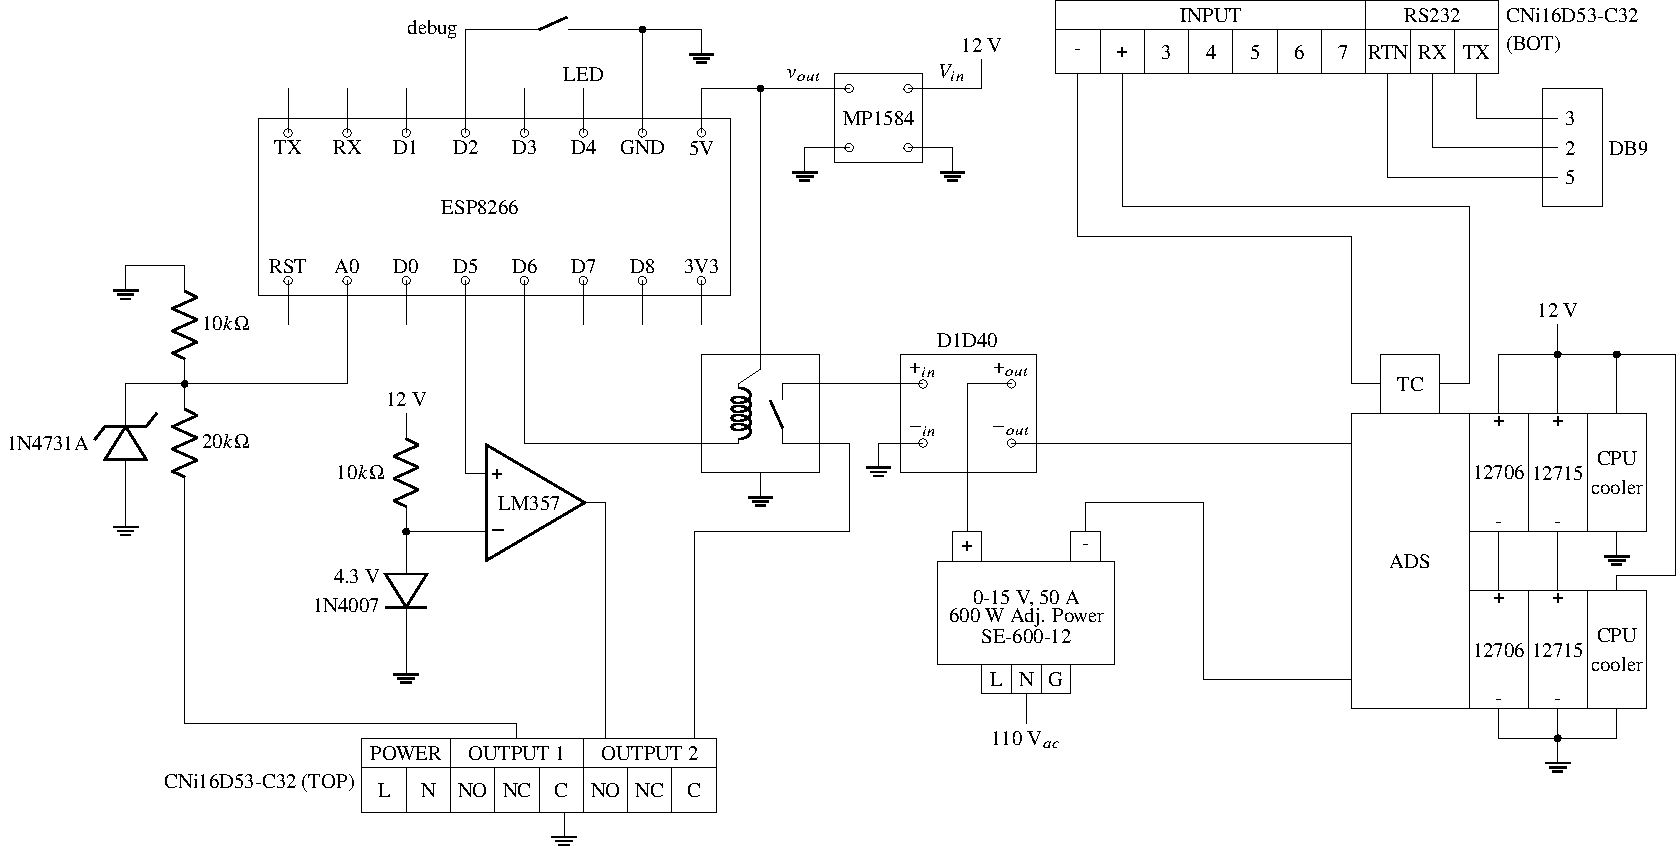
\includegraphics[width=\linewidth]{tikz/ADS heater.pdf}
    \caption{Adsorbent trap heater electronics. The ESP8266 functions as a voltage to PWM converter that adds functionality to the PID controller. PID OUTPUT 2 is a simple relay that prevents the trap from activating without the PID being turned on. Setting OUTPUT 2's set point the maximum allowable temperature of the adsorbent trap adds protection to the trap to prevent overheating.}
    \label{fig:rendered adsorbent trap}
\end{figure}


\subsection{Communications}
\begin{figure}[H]
    \centering
    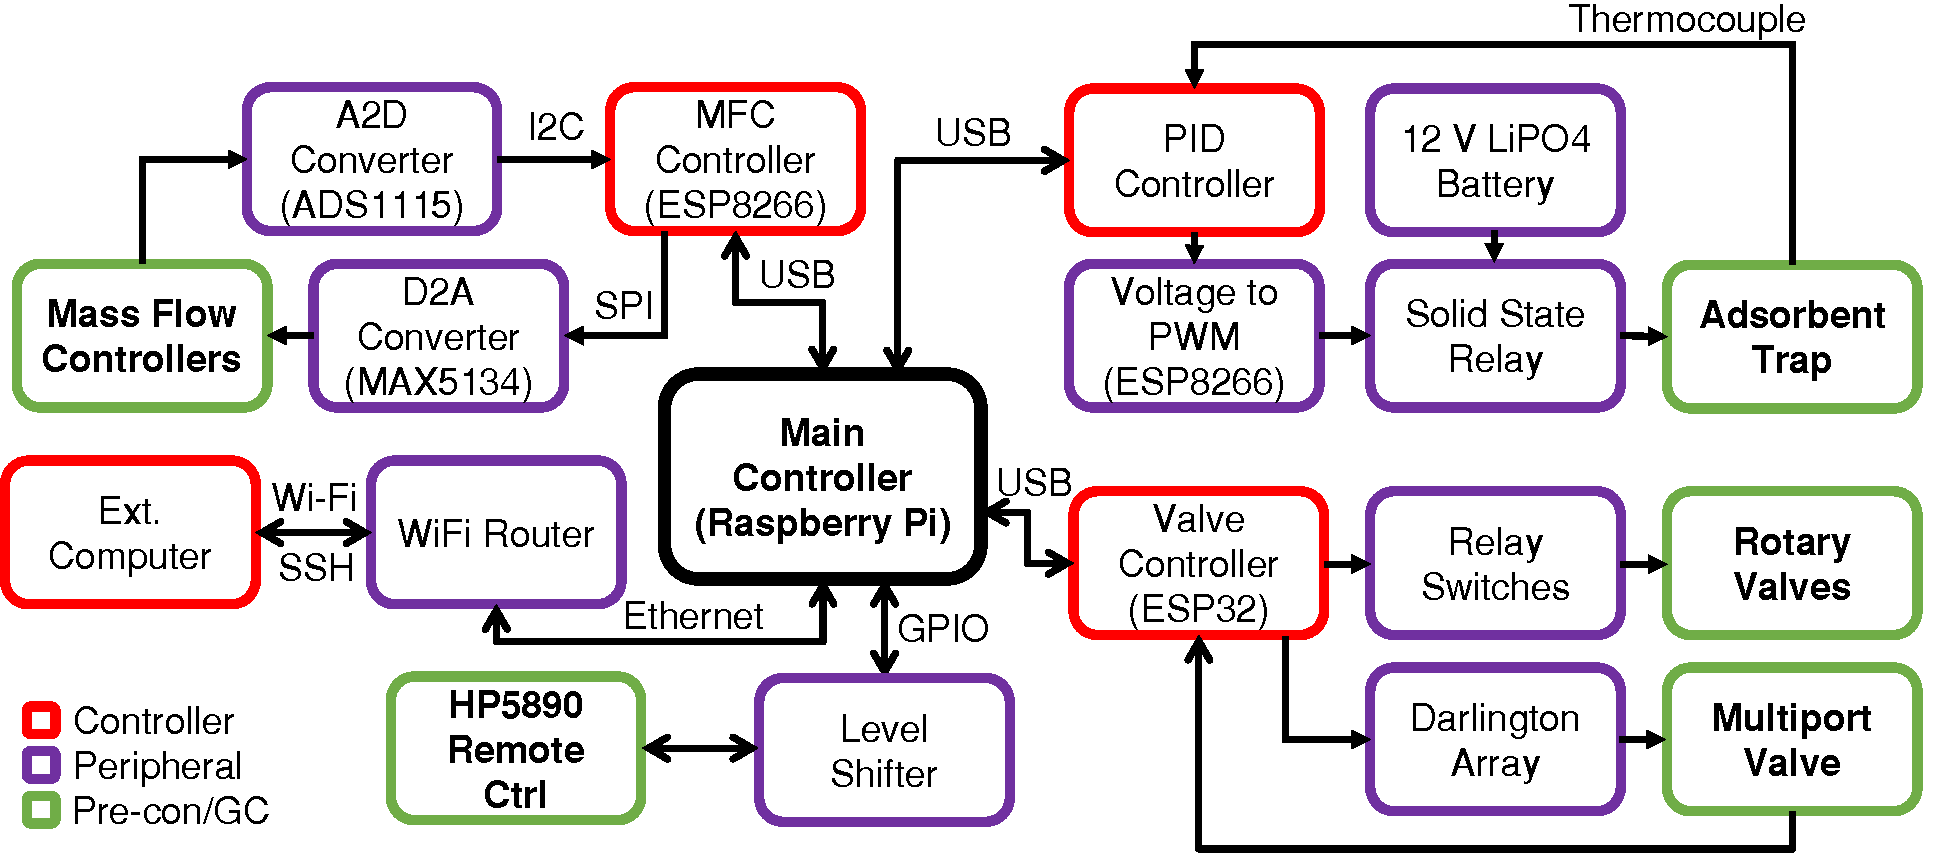
\includegraphics[width=\linewidth]{Figures/Preconcentration Controller Schematic.pdf}
    \caption{Communication diagram showing how the Raspberry Pi interfaces with each component of the pre-concentration system, and the GC.}
    \label{fig:enter-label}
\end{figure}



\end{landscape}
